% -------------------- frame 1 -------------------
\begin{frame}{Serverless}

\begin{itemize}
\item<1-> Serverless computing abstracts the underlying infrastructure, focusing solely on the logic that needs to be performed to solve a given task.

\item<2-> A developer just write a function using their favourite programming language and put it online.

\item<3-> A new concept of Function-as-a-Service.

\item<4-> Edge computing is recommended by setting up compute infrastructure closer to the data source.

\item<5-> It is a new frontier for IoT computing [2].

\end{itemize}
    
\end{frame}

% ----------------- frame 2 ----------------

\begin{frame}{Serverless architecture}
    \begin{figure}
        \centering
        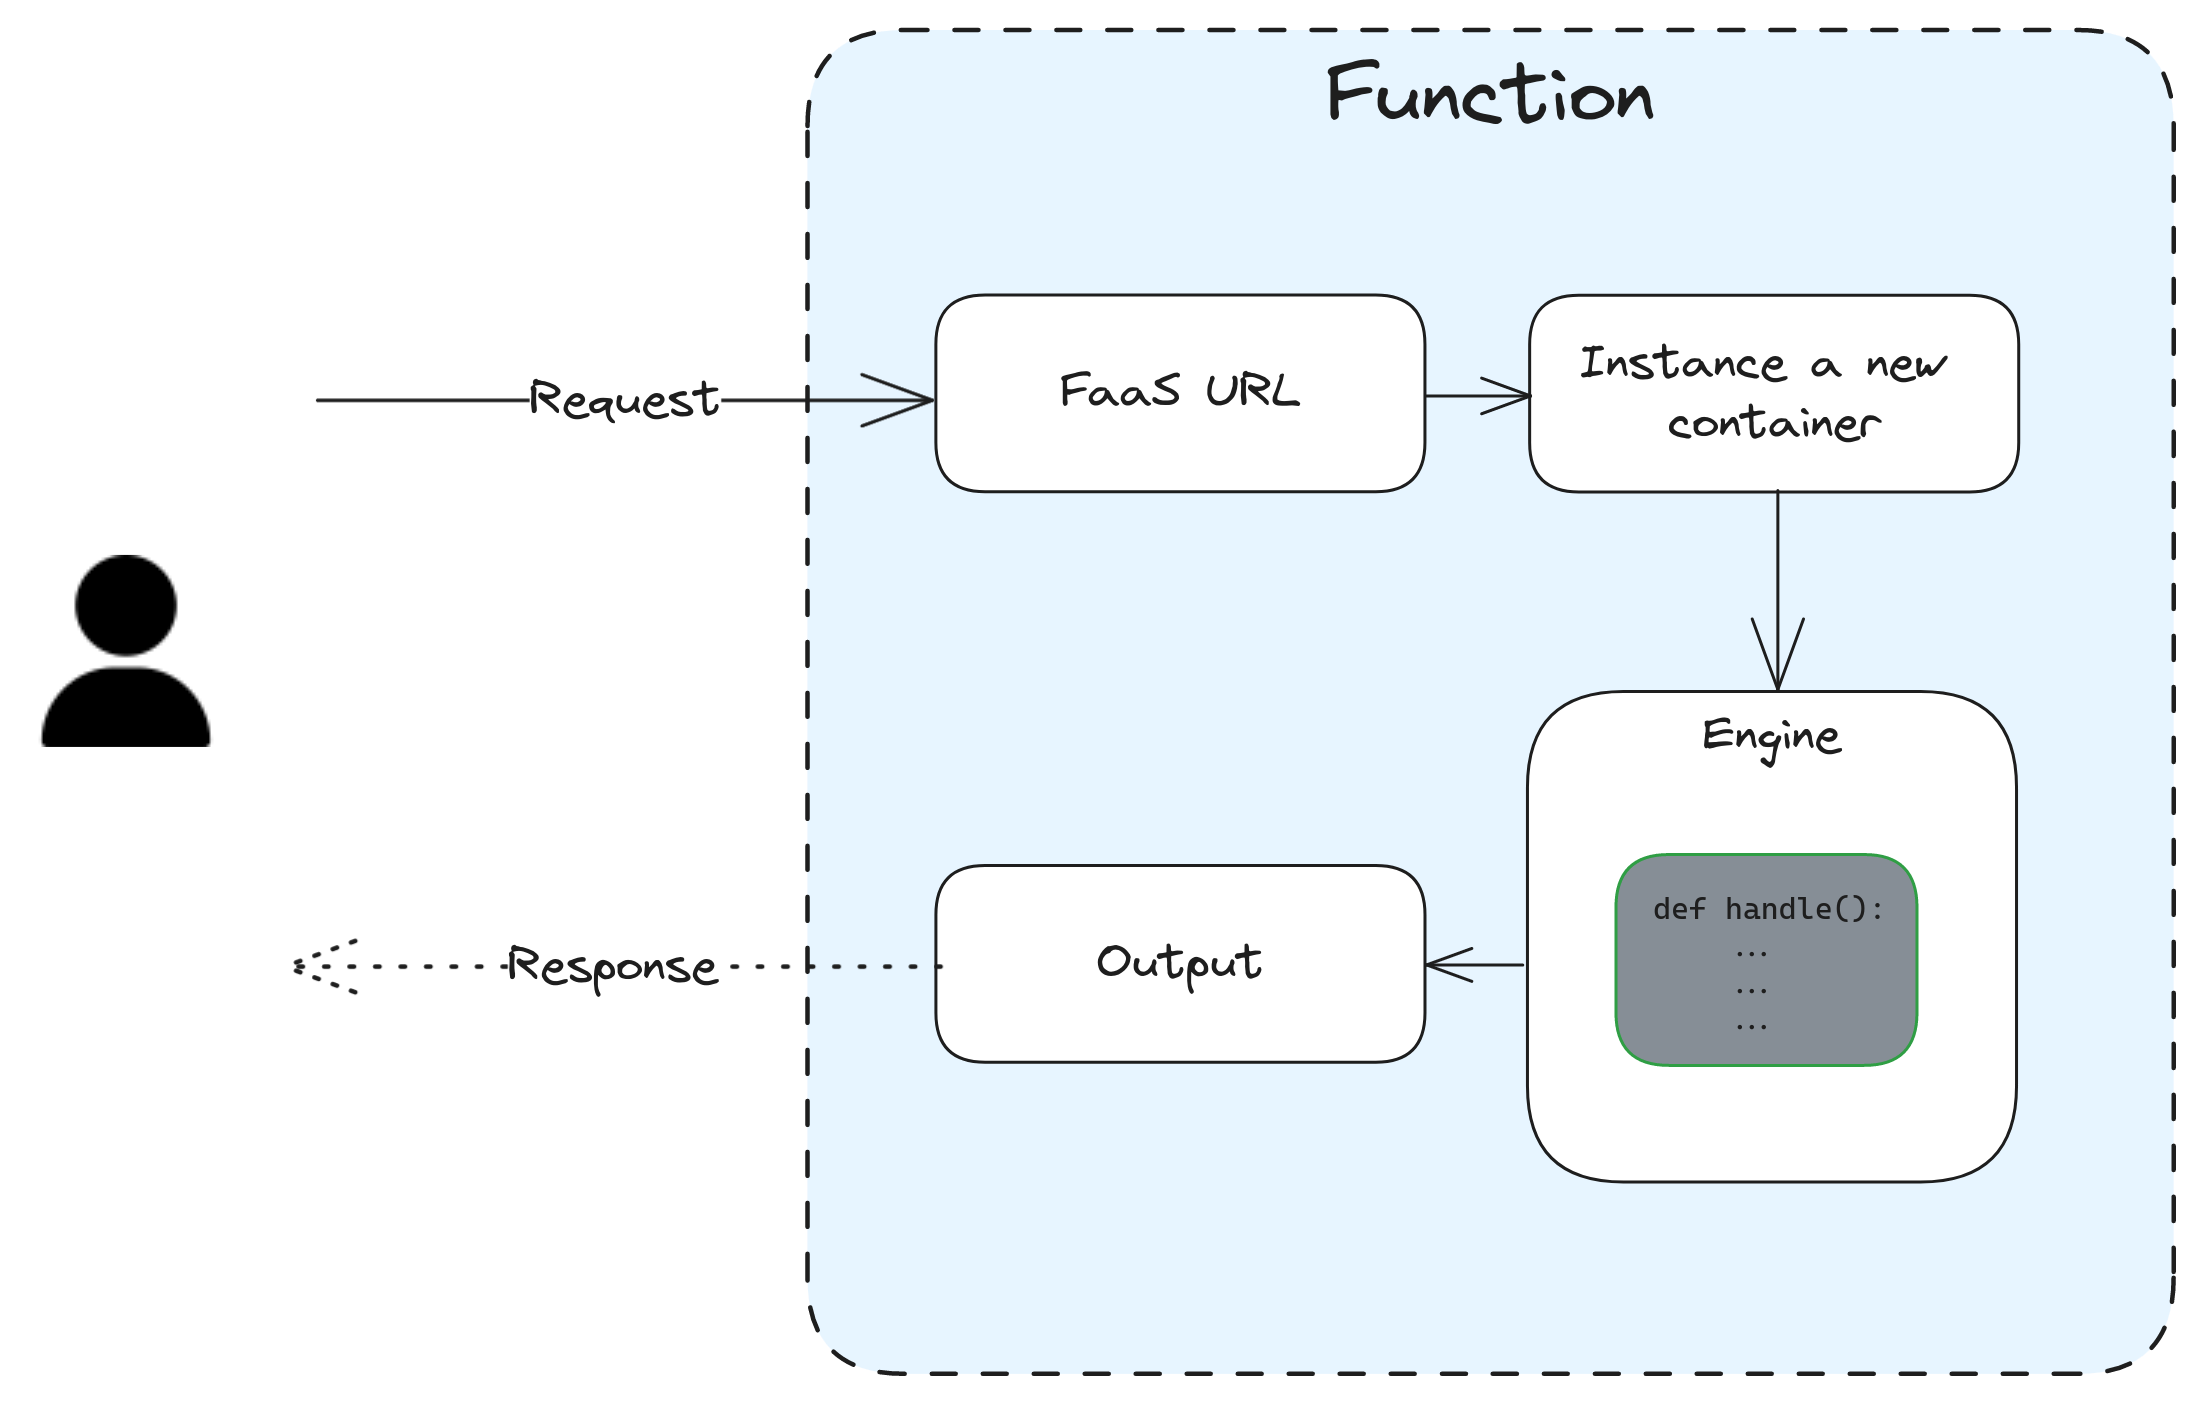
\includegraphics[width=1\linewidth]{static/Untitled-2023-09-27-1503(4).png}
    \end{figure}
\end{frame}

% ------------------ frame 3 ---------------------
\begin{frame}{Serverless platforms}

There is a new market for serverless platforms, both open and closed source.

\begin{itemize}
    \item AWS Lambda
    \item OpenWhisk
    \item Kubeless
    \item Knative
    \item OpenFaaS
\end{itemize}
    
\end{frame}

% ------------------ frame 3 ---------------------
\begin{frame}{Serverless platforms}

There is a new market for serverless platforms, both open and closed source.

\begin{itemize}
    \item AWS Lambda
    \item OpenWhisk
    \item Kubeless
    \item Knative
    \item OpenFaaS \alert{\textit{we chose this one!}}
\end{itemize}
    
\end{frame}

% ---------------- frame 4 ----------------------
\begin{frame}{OpenFaaS}

Its architecture is composed by:

\begin{itemize}
    \item API Gateway
    \item Prometheus [3]
    \item Watchdog
    \item Docker Swarm or Kubernetes
    \item Docker
\end{itemize}

It supports two different function scaling modes:

\begin{itemize}
    \item Native scaling based on internal customized metrics
    \item Kubernetes Horizontal Pod Autoscaler (HPA)
\end{itemize}

\end{frame}